%% Hand-drawn (TikZ) example of ONE generated model, for the reviewer's "show a
%% representative generated architecture, traced to evidence" request. NOT generated by
%% analysis/ -- but every box and arrow below is transcribed 1:1 from a real pipeline
%% output, so re-run the pipeline before editing anything structural here:
%%
%%   subject   GNU bash 4.2 fixture (autotools L0 + Doxygen L2), run of 2026-07-16
%%   source    out/bash/architecture/generated/generated-components.dsl    (12 containers)
%%             out/bash/architecture/generated/generated-relationships.dsl (17 container->container lines)
%%             out/bash/architecture/generated/curated-facts.json          (evidence strings, verbatim)
%%   rules     overlays/bash/architecture/rules/mapping-rules.yaml (5 group: rules; 7 libs unmatched)
%%
%% Fidelity notes (keep these true):
%%  * Container names are the DSL names verbatim. All 17 container->container relationships
%%    of the DSL are drawn; nothing is added. The DSL's other 39 lines are component-altitude
%%    (a `bash`/`basename`/... component is one endpoint, e.g. `bash -> libbuiltins`); they
%%    belong to the component views, not to this container view, and are not drawn.
%%  * Line style = evidence strength from curated-facts.json (model.py compute_confidence):
%%      thick  = "link + include corroborate" (confidence medium)       3 edges
%%      solid  = "link only": declared in the Makefile, no include seen (confidence low, the
%%               plan's "declared but never used" case)                  6 edges
%%      dotted = "include only": not declared in any build file (low)   8 edges
%%  * Dashed boxes = the seven targets whose `tags` carry `needs-curation` in curated-facts
%%    (no mapping rule matched -> provisional singleton). The DSL additionally tags Shell
%%    Core / Example Loadables / Memory Allocator `needs-curation` through the rendering-time
%%    naming-convention lint (spaced names are the minority against seven lowercase lib
%%    names, generate_structurizr._mixed_convention_outliers); that lint is NOT drawn.
%%  * Evidence callouts 1-3 quote the `evidence[].detail` strings verbatim:
%%      1  rel:cpp:target:bash->cpp:target:libbuiltins
%%           link:    Makefile: bash links libbuiltins
%%           include: #include "builtins/common.h" (+16 more)     (count 17)
%%      2  rel:cpp:target:bash->cpp:target:libtermcap
%%           link:    Makefile: bash links libtermcap             (the only evidence)
%%      3  rel:cpp:target:libsh->cpp:target:bash
%%           include: #include "include/stdc.h" (+103 more)       (count 104)
%%  * No edge carries the `suspicious-declared` tag (architecture-drift.md: "_none_");
%%    the "link only" edges are the low-confidence declared-but-unused-in-source kind.
%%
%% Core tikz only (no \usetikzlibrary). Anonymity-safe: no tool name. Drawn at
%% ~9.6 x 6.9 cm for \resizebox{\columnwidth}{!}{...}; the caller wraps it in a figure.
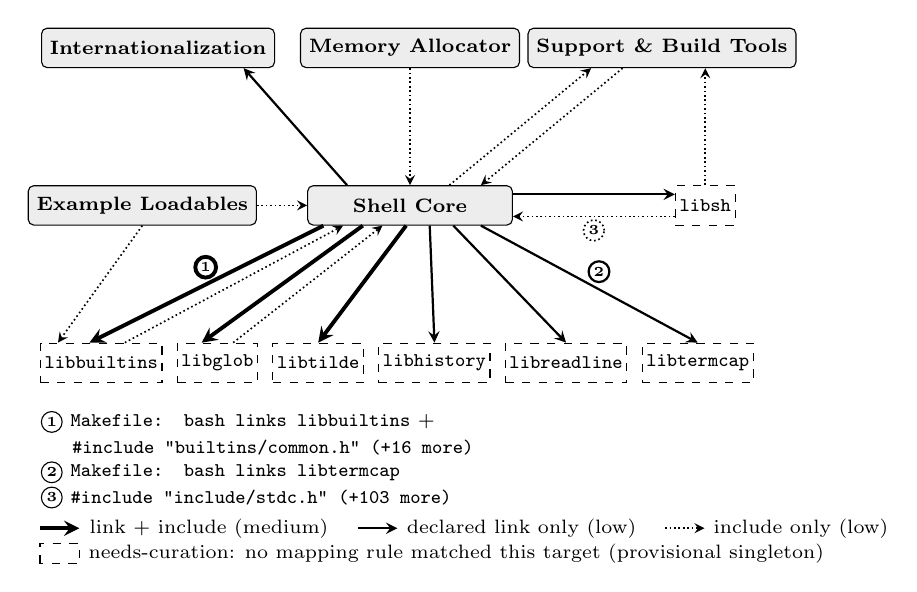
\begin{tikzpicture}[x=1cm,y=1cm,
  % containers: rounded+shaded = curated C executable group; plain = C static library
  exe/.style={draw, rounded corners=2pt, fill=black!7, minimum height=0.5cm,
              inner xsep=3pt, inner ysep=3pt, align=center, font=\scriptsize\bfseries},
  lib/.style={draw, fill=white, minimum height=0.5cm, inner xsep=1.5pt, inner ysep=3pt,
              align=center, font=\scriptsize\ttfamily},
  nc/.style={dashed},                                   % needs-curation (no rule matched)
  % relationships, by evidence strength
  corr/.style={->, >=stealth, line width=1.4pt},        % link + include corroborate (medium)
  link/.style={->, >=stealth, thick},                   % declared link only (low)
  inc/.style={->, >=stealth, densely dotted, semithick},% include only, undeclared (low)
  % evidence callout markers + legend text
  ev/.style={circle, draw, fill=white, inner sep=0pt, minimum size=7.5pt,
             font=\tiny\bfseries},
  leg/.style={font=\scriptsize, inner sep=0pt, anchor=west},
  ]
  % ---- containers (names verbatim from generated-components.dsl) ------------------
  \node[exe] (intl) at (1.65,4.4) {Internationalization};
  \node[exe] (mem)  at (4.85,4.4) {Memory Allocator};
  \node[exe] (sup)  at (8.05,4.4) {Support \& Build Tools};
  \node[exe] (ex)   at (1.45,2.4) {Example Loadables};
  \node[exe] (core) at (4.85,2.4) [minimum width=2.6cm] {Shell Core};
  \node[lib, nc] (libsh) at (8.6,2.4) {libsh};
  % bottom row chained off each other's east anchors (cmtt widths differ per name)
  \node[lib, nc, anchor=west] (libbuiltins) at (0.15,0.4) {libbuiltins};
  \node[lib, nc, anchor=west] (libglob)     at ([xshift=1.8mm]libbuiltins.east) {libglob};
  \node[lib, nc, anchor=west] (libtilde)    at ([xshift=1.8mm]libglob.east)     {libtilde};
  \node[lib, nc, anchor=west] (libhistory)  at ([xshift=1.8mm]libtilde.east)    {libhistory};
  \node[lib, nc, anchor=west] (libreadline) at ([xshift=1.8mm]libhistory.east)  {libreadline};
  \node[lib, nc, anchor=west] (libtermcap)  at ([xshift=1.8mm]libreadline.east) {libtermcap};
  % ---- declared links from the shell core (Makefile LDADD, L0) ---------------------
  \draw[corr] ([xshift=-11mm]core.south) -- ([xshift=-1.5mm]libbuiltins.north)
    node[ev, pos=0.45, xshift=-4.5pt, yshift=4pt] {1};
  \draw[corr] ([xshift=-6mm]core.south)   -- ([xshift=-2mm]libglob.north);
  \draw[corr] ([xshift=-0.5mm]core.south) -- (libtilde.north);
  \draw[link] ([xshift=2.5mm]core.south)  -- (libhistory.north);
  \draw[link] ([xshift=5.5mm]core.south)  -- (libreadline.north);
  \draw[link] ([xshift=9mm]core.south)    -- (libtermcap.north)
    node[ev, pos=0.5, xshift=3.5pt, yshift=4.5pt] {2};
  \draw[link] ([yshift=1.4mm]core.east)   -- ([yshift=1.4mm]libsh.west);
  \draw[link] ([xshift=-8mm]core.north)   -- ([xshift=-4mm]intl.south east);
  % ---- include-only edges (Doxygen L2, no build-file declaration) ------------------
  \draw[inc] ([xshift=3mm]libbuiltins.north) -- ([xshift=-8.5mm]core.south);
  \draw[inc] ([xshift=2mm]libglob.north)       -- ([xshift=-3.5mm]core.south);
  \draw[inc] ([yshift=-1.4mm]libsh.west) -- ([yshift=-1.4mm]core.east)
    node[ev, pos=0.5, below=1pt] {3};
  \draw[inc] (ex.east) -- (core.west);
  \draw[inc] (ex.south) -- ([xshift=-5.5mm]libbuiltins.north);
  \draw[inc] (mem.south) -- (core.north);
  \draw[inc] ([xshift=5mm]core.north) -- ([xshift=-9mm]sup.south);
  \draw[inc] ([xshift=-5mm]sup.south) -- ([xshift=9mm]core.north);
  \draw[inc] (libsh.north) -- (libsh.north |- sup.south);
  % ---- legend: the three quoted evidence entries, then the line key ----------------
  \node[ev] (l1) at (0.30,-0.35) {1};
  \node[leg] at (l1.east) {\ \texttt{Makefile: bash links libbuiltins}\ +};
  \node[leg] at (0.55,-0.67) {\texttt{\#include "builtins/common.h" (+16 more)}};
  \node[ev] (l2) at (0.30,-0.99) {2};
  \node[leg] at (l2.east) {\ \texttt{Makefile: bash links libtermcap}};
  \node[ev] (l3) at (0.30,-1.31) {3};
  \node[leg] at (l3.east) {\ \texttt{\#include "include/stdc.h" (+103 more)}};
  \draw[corr] (0.15,-1.70) -- (0.65,-1.70) node[leg, xshift=3pt] (k1) {link + include (medium)};
  \draw[link] ([xshift=10pt]k1.east) -- ++(0.5,0) node[leg, xshift=3pt] (k2) {declared link only (low)};
  \draw[inc]  ([xshift=10pt]k2.east) -- ++(0.5,0) node[leg, xshift=3pt] (k3) {include only (low)};
  \draw[nc]   (0.15,-2.15) rectangle (0.65,-1.89);
  \node[leg] at (0.76,-2.02) {needs-curation: no mapping rule matched this target (provisional singleton)};
\end{tikzpicture}
